\UseRawInputEncoding
\documentclass{article}

% Language setting
\usepackage[english]{babel}
\usepackage{pmboxdraw}

\usepackage[a4paper,top=2cm,bottom=2cm,left=3cm,right=3cm,marginparwidth=1.75cm]{geometry}

% Useful packages
\usepackage{amsmath}
\usepackage{tabularx}
\usepackage[T1]{fontenc}
\usepackage{graphicx}
\usepackage{listings}
\usepackage[colorlinks=true, allcolors=blue]{hyperref}

\title{Homework 06\\"A two-players guessing game"}

\author{Andrea Panceri 1884749}

\begin{document}
\maketitle

\section{Introduction}
There are three parties: Alice and Bob => the players and Charlie  => a trusted third party. Both players secretly choose a number in \{1, ..., 6\}, let's say A for Alice and B for Bob. Charlie (that doesn't see A and/or B) then generates a number C in \{1, ...,6\}. Each of the three parties provides his number to the other two parties. After this we have three possibilities:\\
\begin{itemize}
  \item if |C - A| < |C - B| \textcolor{red}{Alice wins}
  \item if |C - A| > |C - B| \textcolor{red}{Bob wins}
  \item otherwise, the \textcolor{red}{game is drawn}
\end{itemize}
Both Alice and Bob aim to win. We want to design a protocol that specifying the sequence of messages to be sent. It is important that the parties will respect the rules, but will not hesitate to manipulate them and use them to their advantage in order to benefit from them. Messages sent to the parties will allow them to understand (all three) if there is and who is the winner or if the game is drawn. This are the requisites of the protocol, in the next section we show the implementation.

\section{Protocol Implementations}
Now we start to describe the protocol for the game. For generate a shared key between the players(Alice and Bob) with the trusted server, we will use diffie-hellman. In this way all the information exchanged by the players with the trusted server will be encrypted using the shared keys, and therefore it will not be possible for the other player to obtain sensitive information. For this protocol we use the fact we have a trusted server, given that,we can use the Kerberos protocol for obtain the authentication of Alice and Bob. It is important that Alice and Bob exchange before their values and only after send their values to Charlie, because if a player obtain the value chosen by Charlie at the begin, then he could select a number that guarantee to not loose. While if a player obtain the value chosen from the other player, without knowing the value chosen by Charlie, he can not use this fact in any way. Also it is important to avoid the replay attacks, that a player could use for obtain an easy victory.\\
At first all the three parties randomly generate their values in the range \{1, ..., 6\}. Important now is each  player has a master secret key with the trusted server (obtained with DH), all master keys are stored in the trusted server database, encrypted with the Charlie master key. The value chosen is stored encrypted with the shared key of the player with Charlie.
This part are the same for the two players, we take Alice for example:\\
\begin{enumerate}
   \item Alice send to Charlie: A (identity of Alice), Bob (Other Player identity), N(Nounce).
   \item Charlie sends to Alice: TicketB, K\textsubscript{AC}(K\textsubscript{AB},N, L, B)   'where L is the lifetime of the ticket'.
   \item Now Alice check the nounce and knows the ticket lifetime.\\Alice sens to Bob: TicketB, K\textsubscript{AB}(A,t\textsubscript{A}, VALUE\_CHOSEN\_A)[Authenticator].
   \item Now Bob checks that Alice's identity in TicketB and in Authenticator are the same, and also checks the time validity of ticket.
   \item Bob send to A: K\textsubscript{AB}(t\textsubscript{A},VALUE\_CHOSEN\_B)
\end{enumerate}
We use TicketB = K\textsubscript{BC}(K\textsubscript{AB},A, "Lifetime", timestamp), K\textsubscript{AB} is the session key, "lifetime is the validity of the ticket and t\textsubscript{A} is a timestamp.\\In this way Alice send his value to Bob and vice-versa. After this now the two players send their value to Charlie and Charlie send his vale to the players. Using these messages:\\
\begin{enumerate}
   \item Alice send to Charlie: K\textsubscript{AC}(Alice,t\textsubscript{A},N VALUE\_CHOSEN\_A).
   \item Charlie obtain the value chosen by Alice, but must wait for value of Bob. Charlie sends to Alice: K\textsubscript{AC}(Charlie,N,t\textsubscript{A}, VALUE\_CHOSEN\_C)
   \item Alice obtain the value chosen by Charlie and check the result of the game.
   \item Bob send to Charlie: K\textsubscript{BC}(Bob,t\textsubscript{B},N VALUE\_CHOSEN\_B).
   \item Charlie obtain the value chosen by Bob and check the result of the game. Charlie sends to Bob: K\textsubscript{BC}(Charlie,N,t\textsubscript{B}, VALUE\_CHOSEN\_C)
   \item Bob obtain the value chosen by Charlie and check the result of the game.
\end{enumerate}
In summary, the whole protocol works thanks to the fact that there is a trusted server that shares keys with the players, these keys will be used to maintain the confidentiality of the messages, and also essential for checking the authenticity between the two players with the use of tickets. We have that the protocol is resistant to replay attacks thanks to the use of Nounces, timestamps and the same ticket in which we enter the identity of the other player. As said before the order of the exchange of the chosen values is not negligible, the players must exchange their values between them, then send them to the trusted authority and only at the end get the value chosen by Charlie to know the result of the game.\\ Another possible way to increment security is that Alice doesn't send only his value but also the value chosen by Bob to Charlie, Bob do same thing. Charlie check that the pairs received are the same, check the result and send an ACK to Alice and Bob with the result. Alice and Bob checks that their result are correct. This is an add on, is not necessary, the protocol that we showed already work.\\Now we show an instance of the game, with the message exchanged:\\
\begin{center}
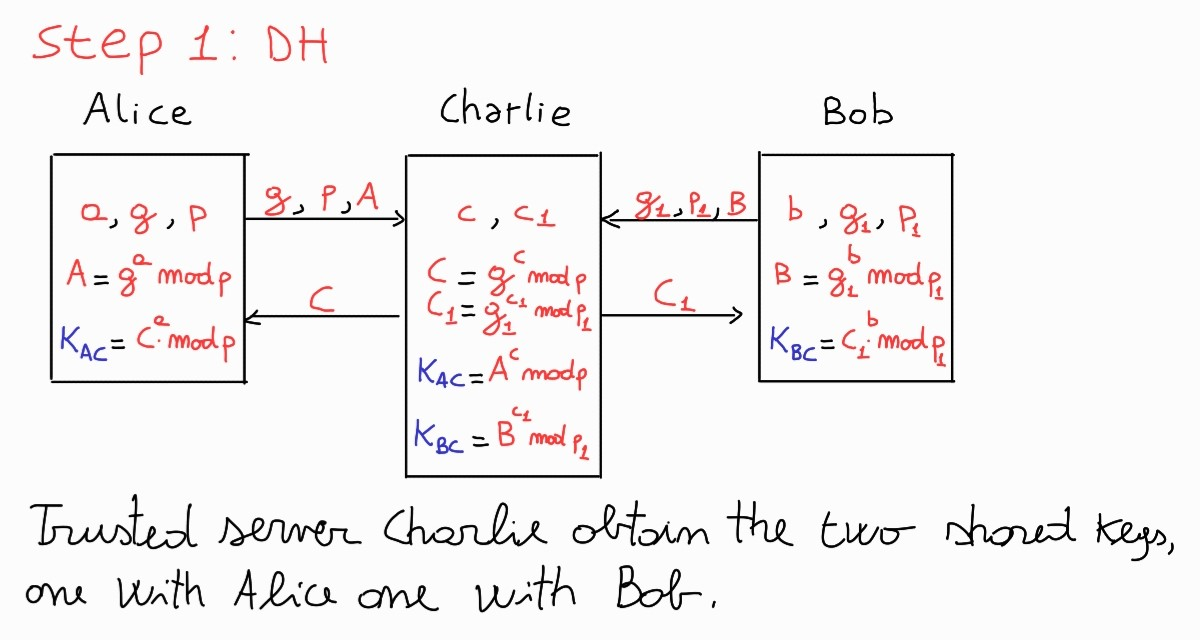
\includegraphics[scale=0.4]{HW06-1884749-2}
\end{center}
\begin{center}
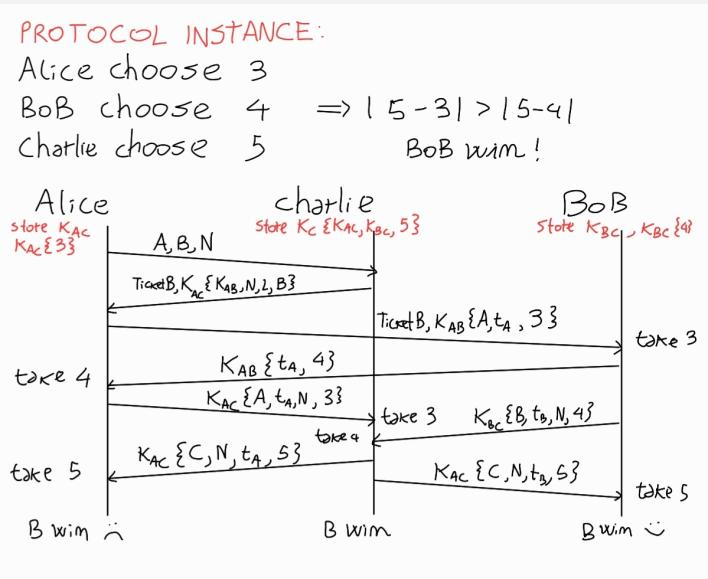
\includegraphics[scale=0.4]{HW06-1884749}
\end{center}
It is also possible to do the same protocol but with less messages, we can use the same assumption that each player has a secret share key with the server. The players send encrypting using his key the value chosen to Charlie. Charlie check the result and send to each player his value and the value chosen by the other player. The only problem can be that the trusted third party advantage one player, but is trusted. For completeness we report the same istance but with the more efficent protocol:\\
\begin{center}
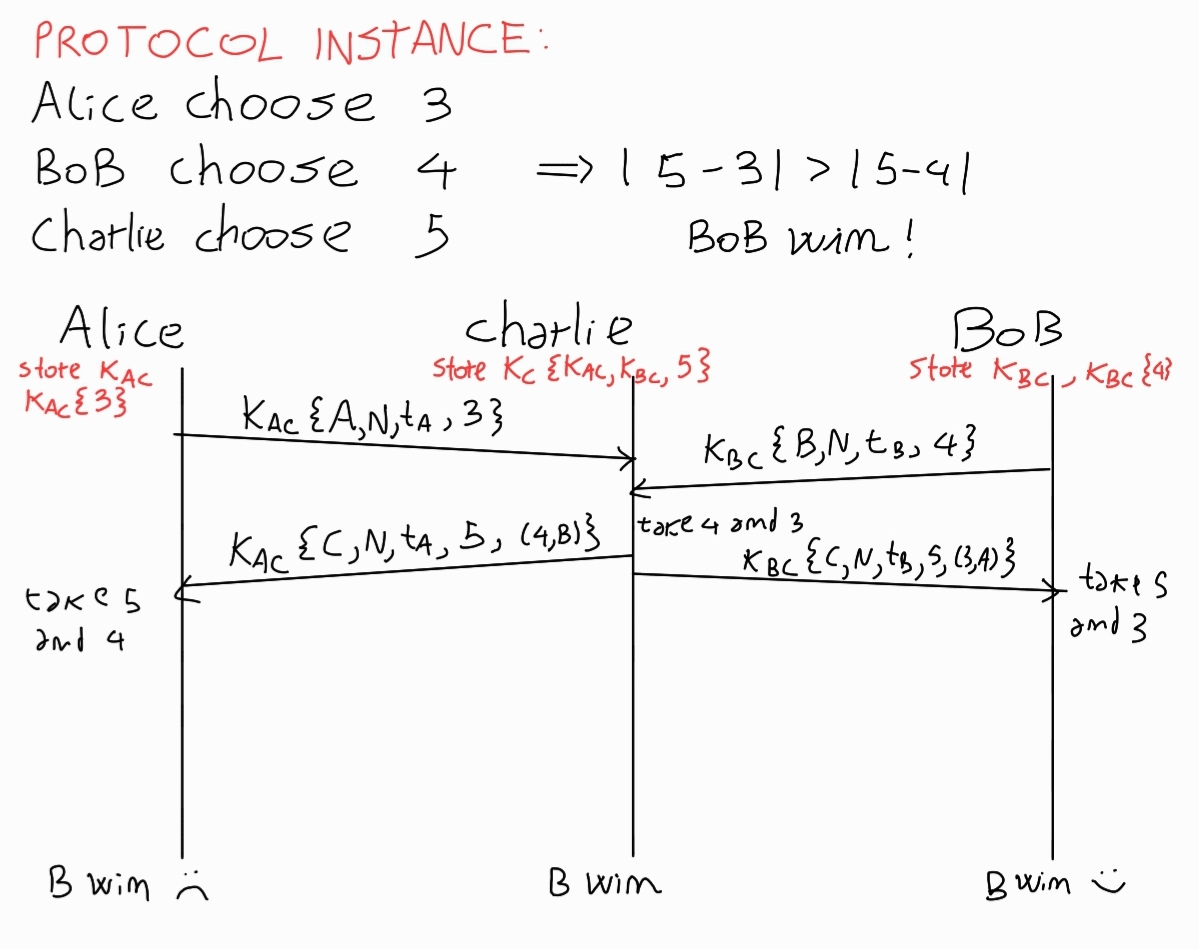
\includegraphics[scale=0.3]{HW06-1884749-1}
\end{center}
All work because a player can distinguish the value of Charlie from the value of the other player, thanks to the fact that Charlie send the value of the other player associated with the identity of the other player. The replay attack don't work because we use the nounce and timestamp, and because in the encrypted message we add the identity of the sender that can not be changed from the attacker if he don't know the private key. Spoofing also is not usefully because the messages are encrypted with the private key.
\end{document}
